\documentclass[10pt,peerreviewca]{IEEEtran} % [11pt,english]{article}
\usepackage[version=4]{mhchem}
\usepackage{siunitx}
\usepackage{physics}
\usepackage{amsmath}
\usepackage{cuted}
\usepackage[justification=centering]{caption}
\usepackage{graphicx}
\graphicspath{ {images/} }

\newcommand{\e}{\mathrm{e}}
\newcommand\numberthis{\addtocounter{equation}{1}\tag{\theequation}}
\newcommand{\opmat}[1]{\mathbf{#1}}

% Some voodoo to fix matrix spacing
\makeatletter
\renewcommand*\env@matrix[1][\arraystretch]{%
  \edef\arraystretch{#1}%
  \hskip -\arraycolsep
  \let\@ifnextchar\new@ifnextchar
  \array{*\c@MaxMatrixCols c}}
\makeatother

\author{
	Lee, Seungsup
	\and
	Miller, Dory
	\and
	Payant, Andrew
	\and
	Powers-Luhn, Justin
	\and
	Zhang, Fan
}

\title{Nuclear Reactor Theory Project \#1\\Group \#3}


\begin{document}
	\pagenumbering{gobble}
	\maketitle
	\newpage
	\pagenumbering{arabic}
	
	\section{Introduction \& Background}
	Proving the capabilities and safety of a reactor design requires effective modeling of the neutron flux in the core (expressed in equation \ref{eqn:transport}). For real cores, however, this is impossible, and must be first simplified, then discretized to provide the solution for a representative mesh. Simplifications that can be applied are: 
	\begin{enumerate}
		\item{\textbf{Isotropic assumption}: ignoring the direction of the incoming neutron. This effectively drops all terms involving $\hat{\Omega}$}
		\item{\textbf{Monoenergetic assumption}: ignoring the energy variance of the neutrons. This means that a single set of cross sections can be used and allows us to ignore neutrons scattering into and out of the domain of interest}
		\item{\textbf{Homogeneity assumption}: assuming that all core materials are evenly mixed throughout the volume of interest. This allows us to ignore discrete boundaries between materials}
		\item{\textbf{Steady-state assumption}: assuming that the system has been in this state for a long period and that no transients occur. This allows us to remove all the time dependent terms.}
	\end{enumerate}

	For this project we have analyzed a simplified, monoenergetic, non-multiplying medium in one dimension. The flux originates from a single source at $x=0$ with a strength of $S=\SI{1E8}{\per\second}$. These assumptions simplify the transport equation to that presented in equation \ref{eqn:simplified_diffusion}.

	In the following sections, we will first describe the terms in equation \ref{eqn:simplified_diffusion}, then provide both an analytical and a discrete solution. We will also provide an analysis of the accuracy of the analysis as a function of the number of nodes. Finally, we will analzye the solution for different coordinate systems to equation \ref{eqn:simplified_diffusion}.

	%\begin{strip}
	\begin{equation}
		\pdv{n}{t} + v \hat{\Omega} \cdot \nabla n + v \Sigma_t n \left( \mathbf{r}, E^\prime, \hat{\Omega}, t \right) = \\ \int_{4\pi} d \hat{\Omega} ^\prime \int_0^{\infty} dE ^\prime v^\prime \Sigma_s\left( E ^\prime \rightarrow E, \hat{\Omega} ^\prime \rightarrow \hat{\Omega} \right) n\left( \mathbf{r}, E ^\prime, \hat{\Omega} ^\prime, t \right) + s\left( \mathbf{r}, E, \hat{\Omega}, t \right)
		\label{eqn:transport}
	\end{equation}
	%\end{strip}

	\begin{equation}
		-D_m \dv[2]{\phi}{x} + \Sigma^m_a \phi = 
		\begin{cases}
			S & \left(x=0\right) \\
			0 & \left(x>0\right)
		\end{cases}
		\label{eqn:simplified_diffusion}
	\end{equation}

	\begin{table*}
		\begin{center}
		\begin{tabular}{ c c c c c }
			\hline
			\textit{Material} & $ \Sigma_{tr}(\si{cm^{-1}}) $ & $ \Sigma_a (\si{cm^{-1}}) $ & $ \nu \Sigma_f (\si{cm^{-1}}) $ & \textit{Relative Absorption} \\
			\hline
			\ce{H} & \num{1.79e-2} & \num{8.08e-3} & 0 & \num{0.053} \\
			\ce{O} & \num{7.16e-3} & \num{4.90e-6} & \num{0} & \num{0}\\
			\ce{Zr} & \num{2.91e-3} & \num{7.01e-4} & \num{0} & \num{0.005} \\
			\ce{Fe} & \num{9.46e-4} & \num{3.99e-3} & \num{0} & \num{0.026} \\
			\ce{^{235}U} & \num{3.08e-4} & \num{9.24e-2} & \num{0.145} & \num{0.602} \\
			\ce{^{238}U} &\num{6.95e-3} & \num{1.39e-2} & \num{1.20e-2} & \num{0.091} \\
			\ce{^{10}B} & \num{8.77e-6} & \num{3.41e-2} & \num{0} & \num{0.223} \\
			\hline
			& \num{3.62e-2} & \num{0.1532} & \num{0.1570} & \num{1.000} \\
			\hline
		\end{tabular}
		\label{materials_table}
		\caption{Macroscopic Cross Sections}
		\end{center}
	\end{table*}

	\section{Methodology}
	Equation \ref{eqn:simplified_diffusion} is a simplified description of neutron diffusion through a finite medium, similar to a point source travelling through a shielding material to a detector. The flux, therefore, depends on the transport cross section. This is accounted for in the term $D_m$, which is related to the transport coefficient by $D_m = 3 \Sigma_{tr}^{-1}$. Values for $\Sigma_{tr}$ for typical reactor materials are found in table \ref{materials_table}. 

	\subsection{Analytic Solution}
	In the slab, equation \ref{eqn:simplified_diffusion} is equal to $0$, $-D_m \pdv[2]{\phi}{x} + \Sigma^m_a \phi = 0 $. In order to better group constants, specify a diffusion length, $L = \sqrt{D_m / \Sigma_{a}}$. We can then solve for $\phi(x)$:
	\begin{align*}
		\pdv[2]{\phi}{x} - \frac{\phi}{L} &= 0 \\
		\phi(x) &= A \e^{-x/L} + C \e^{x/L} \numberthis \label{eqn:generalsolution}
	\end{align*}
	First use the boundary condition $\phi(w)=0$ to solve for $C$
	\begin{align*}
		0 &= A \e^{-w/L} + C \e^{w/L} \\
		C &= -A \e^{2w/L} \\
	\end{align*}
	Next, use the fact that $ -D_m \phi^\prime(0) = J(0) = S/2$ to solve for $A$
	\begin{align*}
		J(0) = \frac{S}{2} &= -\frac{A}{L} \left( 1 + \e^{-2w/L} \right) \numberthis \label{eqn:leftboundary} \\
		A &= \frac{S L}{2 D_m}\left( 1 + \e^{-2w/L} \right)^{-1}
	\end{align*}
	Substituting this in to equation \ref{eqn:generalsolution}, we get:
	\begin{equation*}
		\phi(x) = \frac{S L}{2 D_m} \left( \frac{\e^{-x/L} - \e^{\left(x-2w\right)/L}}{1 - \e^{-2w/L}} \right) \numberthis \label{eqn:analyticcartesian}
	\end{equation*}

	\subsection{Numerical Approximation} \label{ssec:numerical}
	It is rare to be faced with a design that allows for an analytical solution. Fortunately, numerical analysis methods exist that allow for approximation of the analytical solution. By dividing our hypothetical medium into discrete sections with nodes at the boundaries between these sections, it is possible to express the flux vector with equation \ref{eqn:linalg_flux}:
	\begin{equation}
		\opmat{A} \vec{\phi} = \vec{S}
		\label{eqn:linalg_flux}
	\end{equation}
	where $\vec{\phi}$ is the flux at each node. The operator $\opmat{A}$ can be derived using the two-node approximation of the  second derivative formula:
	
	\begin{equation*}
		\left. \pdv[2]{\phi}{x} \right|_i \approx \frac{\phi_{i-1} - 2\phi_i + \phi_{i+1}}{\Delta x^2}
	\end{equation*}

	For non-edge nodes, this can be derived as follows:
	\begin{align*}
		-D_m \dv[2]{\phi}{x} &+ \Sigma_a \phi = 0 \\
		-D_m \int_{x_i - \frac{\Delta x}{2}}^{x_i + \frac{\Delta x}{2}} \dv[2]{\phi}{x} dx &+ 
			\int_{x_i - \frac{\Delta x}{2}}^{x_i + \frac{\Delta x}{2}} \Sigma_a \phi dx = 0 \\
		-D_m \left. \dv{\phi}{x} \right|_{x_i - \frac{\Delta x}{2}}^{x_i + \frac{\Delta x}{2}} &+ 
			\int_{x_i - \frac{\Delta x}{2}}^{x_i + \frac{\Delta x}{2}} \Sigma_a \phi dx = 0 \\
		-D_m \left( \frac{\phi_{i+1} - \phi_i}{\Delta x} - \frac{\phi_{i} - \phi_{i-1}}{\Delta x} \right) &+
			\int_{x_i - \frac{\Delta x}{2}}^{x_i + \frac{\Delta x}{2}} \Sigma_a \phi dx = 0 \\
		-D_m \left( \frac{\phi_{i+1} - \phi_i}{\Delta x} - \frac{\phi_{i} - \phi_{i-1}}{\Delta x} \right) &+
			\Sigma_a \phi_i \Delta x = 0
		\intertext{Dividing each term by $\Delta x$ gives:}
		\left( \frac{-D_m}{\Delta x^2} \right) \phi_{i-1} + \left( \frac{2D_m}{\Delta x^2} + \Sigma_a \right)\phi_i + \left( \frac{-D_m}{\Delta x^2} \right) \phi_{i+1} = 0
	\end{align*}
	From this we see that our operator $\opmat{A}$ will have non-corner terms:
	\[
	\begin{bmatrix}[1.5]
		\hdotsfor{5} \\
		\frac{-D_m}{\Delta x^2} & \frac{2D_m}{\Delta x^2} + \Sigma_a & \frac{-D_m}{\Delta x^2} & 0 & \dots \\
		0 & \frac{-D_m}{\Delta x^2} & \frac{2D_m}{\Delta x^2} + \Sigma_a & \frac{-D_m}{\Delta x^2} & \dots \\
		& & \ddots & & \\
		\dots & 0 & \frac{-D_m}{\Delta x^2} & \frac{2D_m}{\Delta x^2} + \Sigma_a & \frac{-D_m}{\Delta x^2} \\
		\hdotsfor{5}
	\end{bmatrix}
	\]
	We then solve for our top row using the boundary condition in equation \ref{eqn:leftboundary}: 
	\begin{align*}
		-D_m \frac{\phi_1 - \phi_0}{\Delta x} + D_m \left. \dv{\phi}{x} \right|_0 + \int_0^{\Delta x / 2} 
			\Sigma_a \phi dx = 0 \\
		-D_m \frac{\phi_1 - \phi_0}{\Delta x} + D_m \frac{S}{2} + \int_0^{\Delta x / 2} 
			\Sigma_a \phi dx = 0 \\
		-D_m \frac{\phi_1 - \phi_0}{\Delta x} + D_m \frac{S}{2} + \Sigma_a \phi_0 \int_0^{\Delta x / 2}
			dx = 0 \\
	\intertext{Divide by $\Delta x$ on both sides:}
		-D_m \frac{\phi_1 - \phi_0}{\Delta x^2} - \frac{S}{2 \Delta x} + \frac{1}{2} \Sigma_a \phi_0 = 0 \\
		\frac{-D_m}{\Delta x^2} \phi_1 + \left( \frac{D}{\Delta x^2} + \frac{1}{2} \Sigma_a \right) \phi_0 = 0
	\end{align*}
	This gives a final matrix $\opmat{A}$ (for $n=5$ nodes):
	\[
	\begin{bmatrix}[1.5]
		\frac{D_m}{\Delta x^2} + \frac{1}{2}\Sigma_a & \frac{-D_m}{\Delta x^2} & 0 & 0 \\
		\frac{-D_m}{\Delta x^2} & \frac{2D_m}{\Delta x^2} + \Sigma_a & \frac{-D_m}{\Delta x^2} & 0 \\
		0 & \frac{-D_m}{\Delta x^2} & \frac{2D_m}{\Delta x^2} + \Sigma_a & \frac{-D_m}{\Delta x^2} \\
		0 & 0 & \frac{-D_m}{\Delta x^2} & \frac{2D}{\Delta x^2} + \Sigma_a
	\end{bmatrix}
	\]

	Additional analysis was performed assuming the presence of a source of strength $f \times S$ located at $x=W$. This produced an operator with matrix values
	\begin{align*}
		a_{\left( n, n \right)} &= BLOOB \\
		a_{\left( n, n-1 \right)} &= BLOOOP
	\end{align*}

	\section{Results}
	A Fortran program was developed to implement the discrete solution to the transport equation from section \ref{ssec:numerical}. The source code is included as an attachment to this report. The numerical solution produced values that converged as the number of nodes increased, showing clearly exponential behavior as $n\rightarrow\infty$. This behavior can be seen in figures \ref{fig:numerical_vs_analytical} and \ref{fig:many nodes one chart}. 

	We have also examined this solution analytically in different coordinate systems, specifically cartesian, cylindrical, and spherical. The output of these solutions is easily seen in figure \ref{fig:different coordinate systems}. Of note, the derivation for spherical coordinates did not allow for incorporation of the boundary condition $\phi(W)=0$, which may account for the difference in that curve. 

	\begin{figure}
		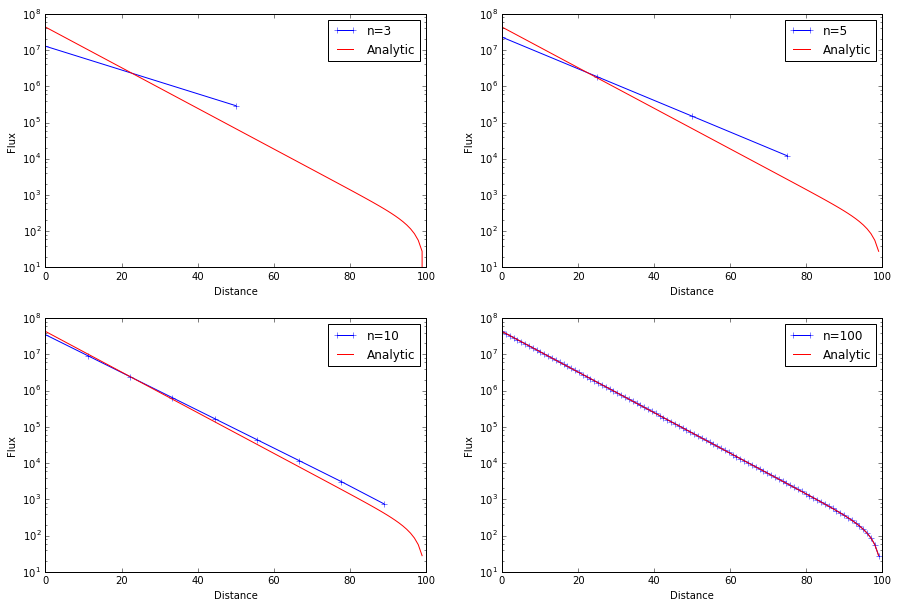
\includegraphics[width=7in]{analytic_vs_numerical}
		\caption{Comparison of Numerical and Analytical Solutions}
		\label{fig:numerical_vs_analytical}
	\end{figure}

	\begin{figure}
		\begin{centering}
		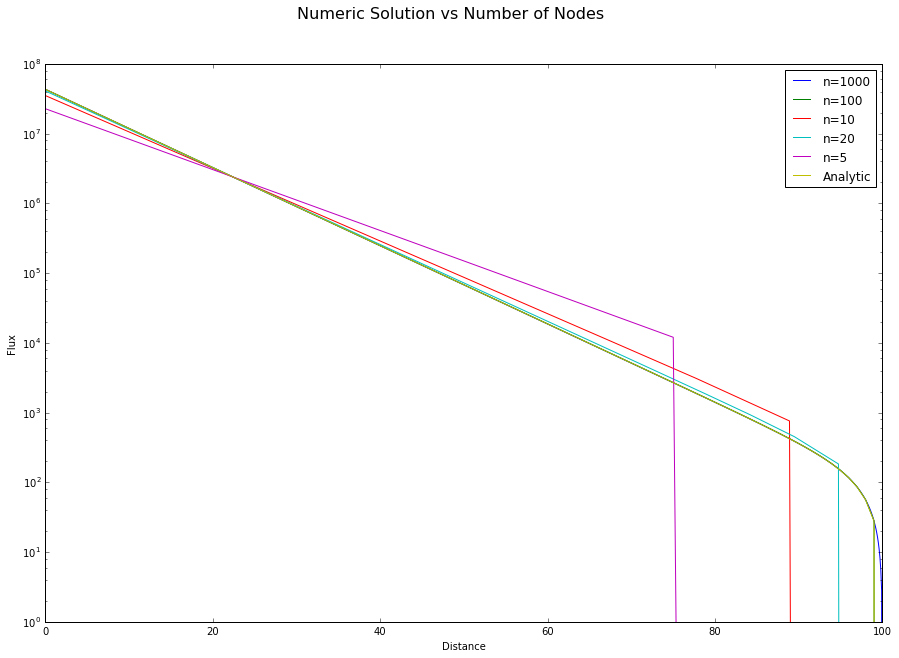
\includegraphics[width=4in]{flux_vs_nodes_one_graph}
		\caption{Change in solution based on number of nodes}
		\label{fig:many nodes one chart}
		\end{centering}
	\end{figure}

	\begin{figure}
		\begin{centering}
		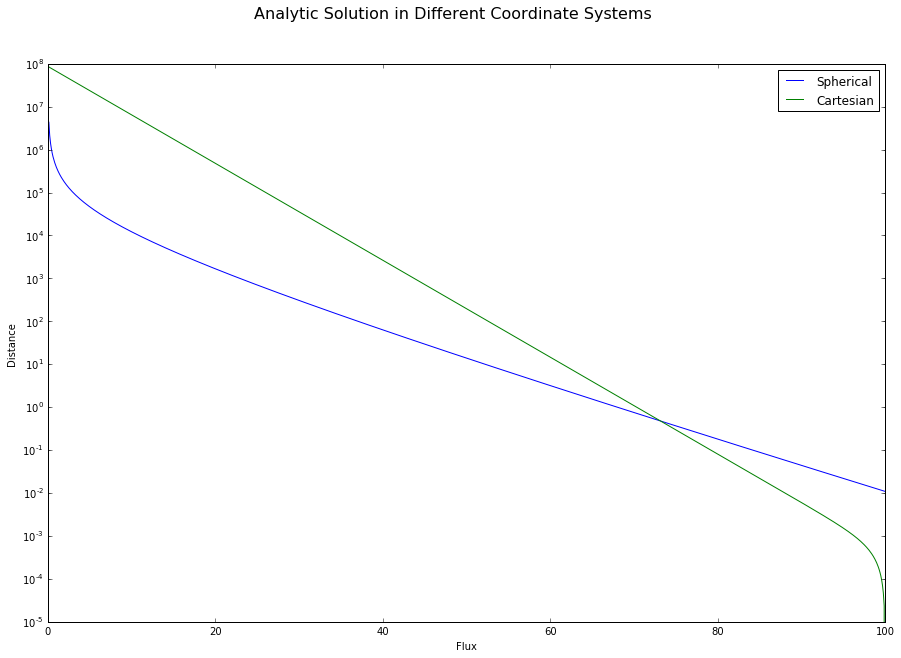
\includegraphics[width=4in]{different_coordinate_systems}
		\caption{Analytical Solution for Cartesian and Spherical Coordinates}
		\label{fig:different coordinate systems}
		\end{centering}
	\end{figure}
	
	\section{Conclusions}
	We provide an analysis of a simplified one-group, one-dimensional neutron diffusion in a non-multiplying medium. Solutions are compared in assorted coordinate systems and for numerical approximation of the analytic solution. The various approaches to this problem produced similar but slightly different solutions, implying that careful choice of methodology is necessary in solving similar problems. 



\end{document}
